\documentclass{article}
\usepackage{tikz, comment}
\usepackage{pifont}
\usepackage{fontspec, pgfplots}
\usetikzlibrary{arrows, decorations.markings, decorations.pathreplacing}
\begin{comment}
:Title: Not defined yet
:Tags: cross product;triple (scalar) product;moment;circumcenter;point of division formula
:Prob: 0.5055;0.3718;0.3392;0.3306;0.3155
:Author: Prof.Hu Ji-shan, HKUST
:Slug: No name yet

Description Here.........
\end{comment}
\begin{document}\centering 

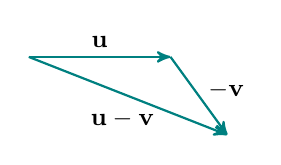
\begin{tikzpicture}[>=latex,xscale=.5*1.8, yscale=.5*1.8][font=\sf\small] 

\draw[teal, thick, ->, >=stealth'] (0, 0) -- (2, 0)node[black, above, midway, pos=0.5, xshift=0, yshift=0, scale=1]{$\bf u$}; %u

\begin{scope}[xshift=2cm,yshift=0cm]
\draw[teal, thick, ->, >=stealth'] (0, 0) -- (0.8, -1.1)node[black, right, midway, pos=0.5, xshift=0, yshift=2, scale=1]{$\bf -v$}; %-v
\end{scope}

\draw[teal, thick, ->, >=stealth'] (0, 0) -- ({2+0.8}, {0-1.1})node[black, below, midway, pos=0.5, xshift=-2, yshift=-2, scale=1]{$\bf u-v$};

\end{tikzpicture}
\end{document}